Let us focus again on a fluid particle, as we did on \ref{sec:}, but
now focusing on how the particle itself distorts as a consequence of a
velocity field.

All possible distorsions of a particle will be a combination of the
following:
\begin{enumerate}
 \item Translation
 \item Rotation
 \item Shear
 \item Dilation
\end{enumerate}

A translation is just the motion of its center of mass from one place
to another, and for a small time is given simply by $\bfu dt$. The
other motions are more complicated, since they involve spatial
derivatives of the velocity. They must: for a constant velocity field
translation is the only mode that occurs.

\subsubsection{Rotation}

We will refer to particle in figure \ref{fig:}, with vertices A, B,
and C. Vertex D plays no role --- also, it is sufficient to focus on
the face that is portrait, even if the shape of a particle is supposed
to be a cube. It is straightfoward to include the other faces, as we
will see.

After a small time $d$ the particle has distorted, so that the
vertices are now at positions A', B', C', and D'.

\begin{figure}
  \centering
  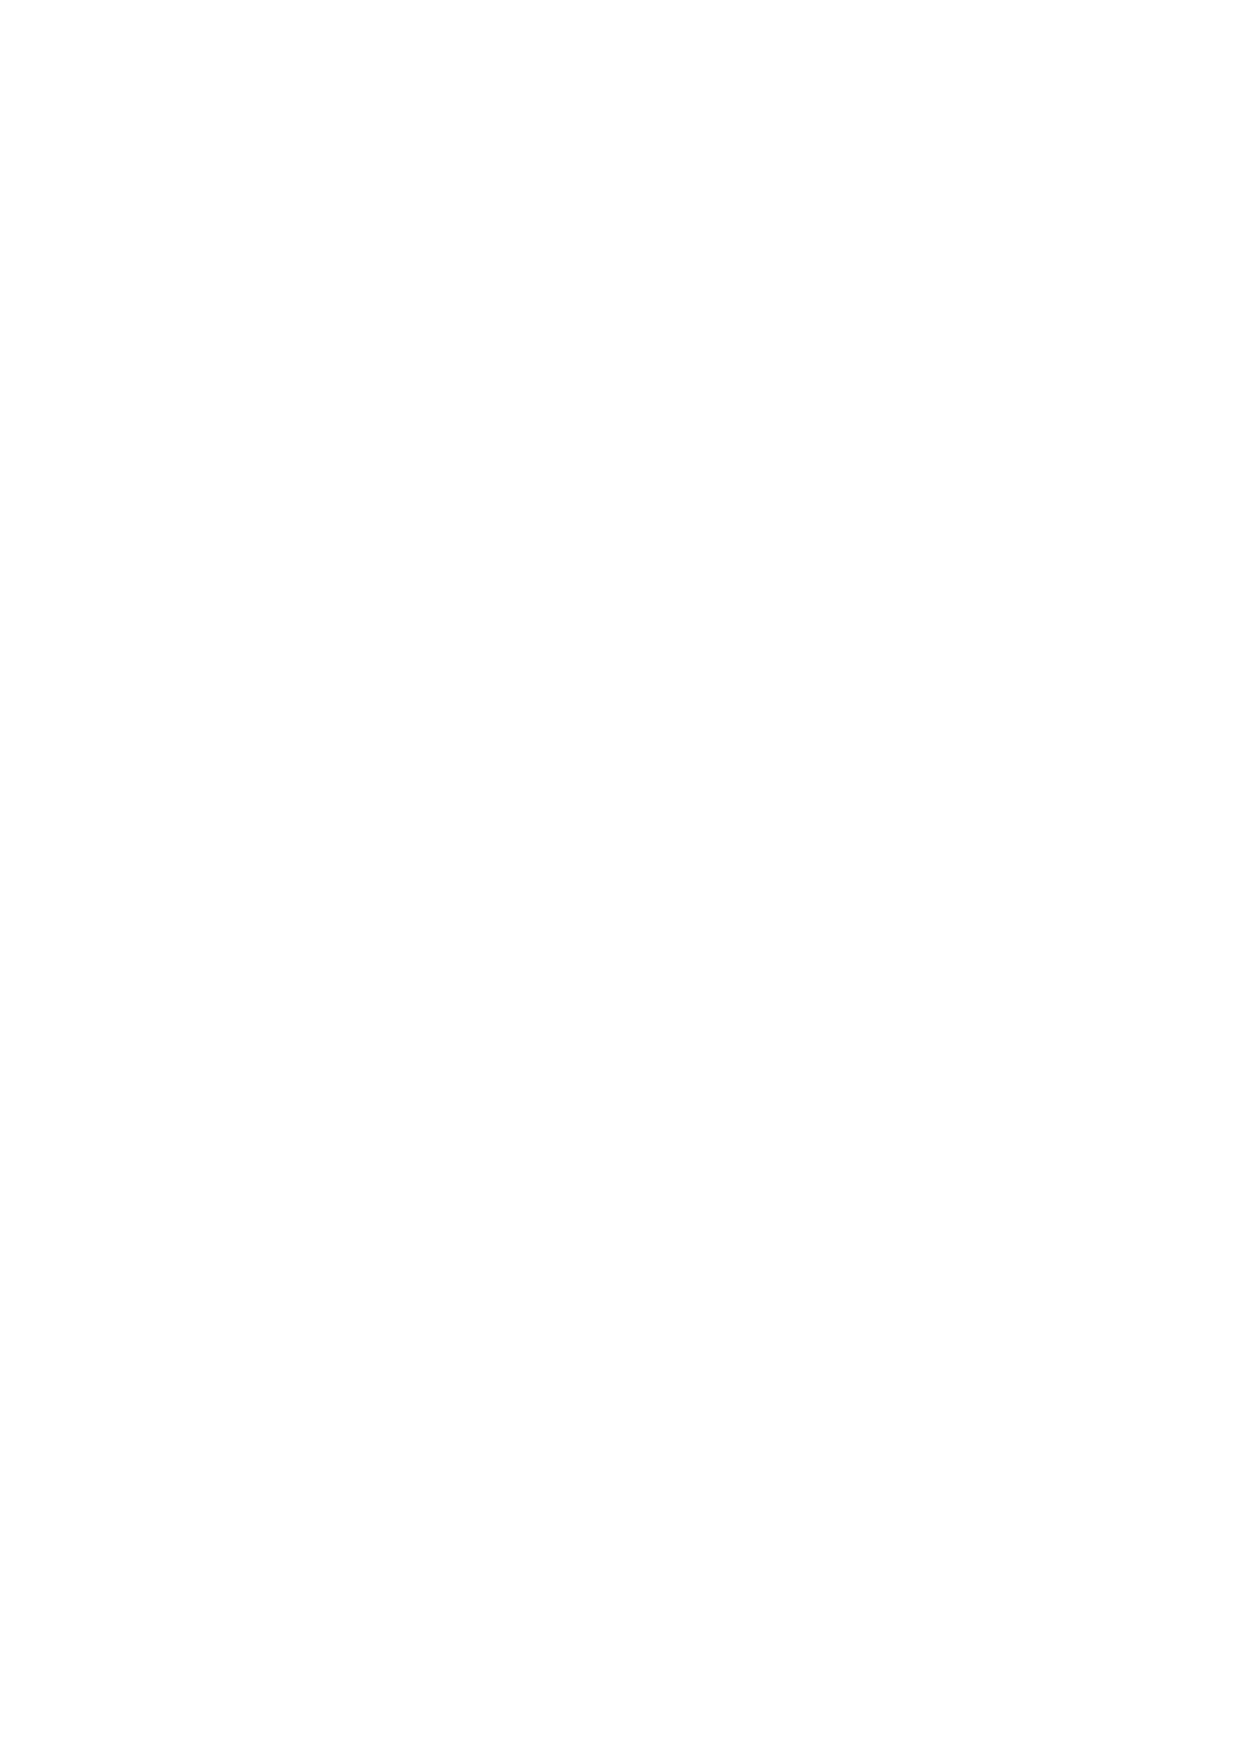
\includegraphics[width=0.4\linewidth]{figures/particle0}
  \caption{\label{fig:particle0}}
\end{figure}



Let us call $\alpha$ the angle between the $x$ axis and the A'-B'
edge, with the usual counter-clockwise convention as
positive. Similarly, $\beta$ is the angle between the A'-C' edge and
the $y$ axis, with the same convention. It is obvious that a net
rotation takes place if e.g. both angles are positive. If, on the
other hand, they are equal in magnitude but differ in sign, no
rotation takes place. This makes it reasonable to define the
rotation as the average of both angles:
\[
d\Omega_z = \frac12
\left(
        \alpha + \beta
\right) .
\]

Now, angle $\alpha$ will always be very small as $dt$ gets very
tiny. Hence, we may approximate it by its tangent:
\[
\alpha \approx \frac{d\ell}{dx'}
\]



\begin{figure}
  \centering
  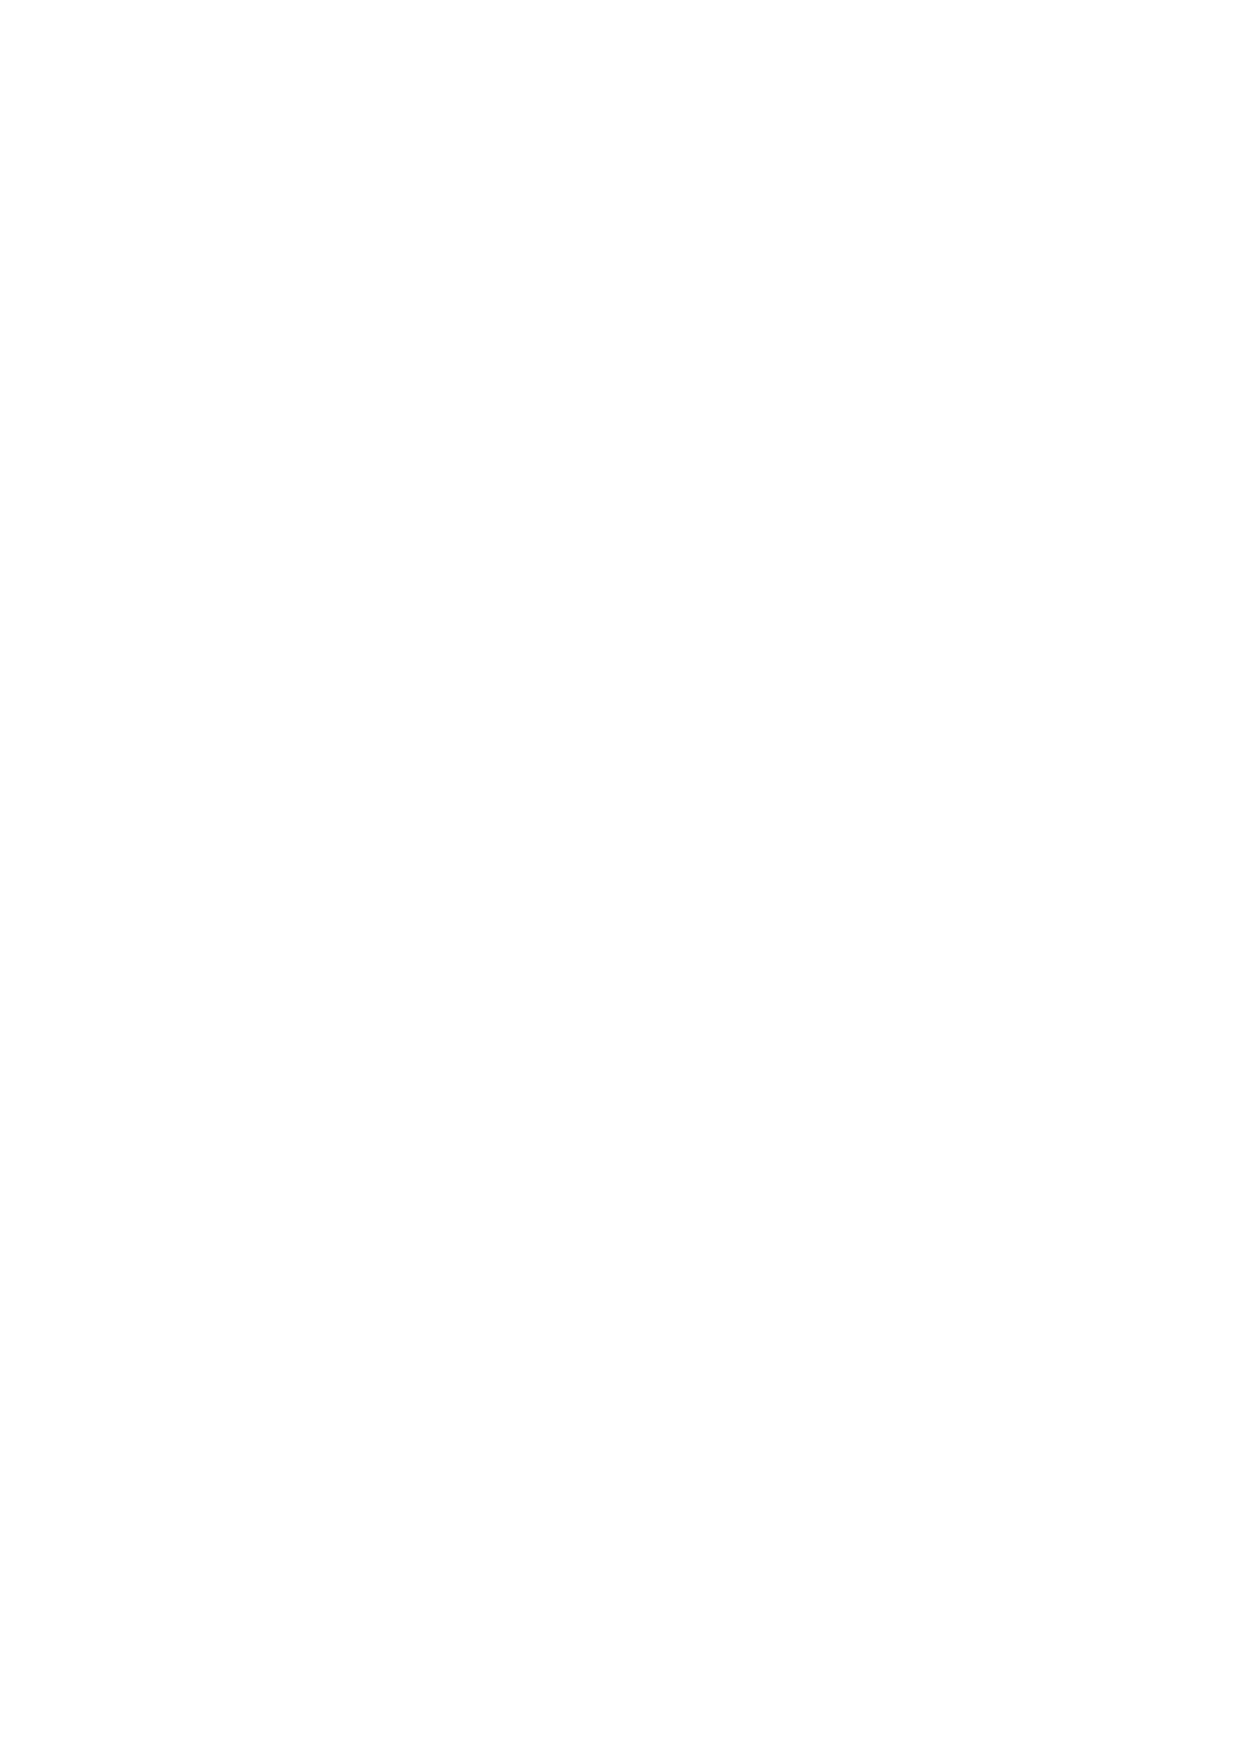
\includegraphics[width=0.4\linewidth]{figures/particle1}
  \caption{\label{fig:particle1}}
\end{figure}

For a small time, we have the following:
\[
dx'=x(B')-x(A') \approx
(dx+v_x(B) dt) - v_x(A) dt \approx
dx+
\left(
v_x(A) +
\frac{\partial v_x}{\partial x} dx
\right ) dt - v_x(A) dt = dx + \frac{\partial v_x}{\partial x} dx dt ,
\]
where we have taken the origin to coincide with the position of A. The
partial derivative is supposed to be evaluated at A, but in the limit
as $dx$ goes to zero it is just ``at the particle''. Similarly, the opposing
side is:
\[ 
d\ell = y(B')-y(B) \approx
v_y(B) dt \approx
\left(
v_y(A) +
\frac{\partial v_y}{\partial x} dx
\right ) dt = \frac{\partial v_y}{\partial x} dx dt ,
\].

Therefore, to first order in $dt$:
\[
\alpha \approx \frac{\partial v_y}{\partial x}  dt .
\]
In other words, the rate of change of the angle is
\[
\frac{d \alpha}{dt} = \frac{\partial v_y}{\partial x}  .
\]
Notice the cross derivative: what is relevant is the change of the
vertical component of the velocity with the horizontal coordinate.

A similar calculation for the other angle reveals
\[
\frac{d \beta}{dt} = - \frac{\partial v_x}{\partial y}  .
\]

Taking all
\[
\frac{d\Omega_z}{dt} = \frac12
\left(
  \frac{\partial v_y}{\partial x}  -
  \frac{\partial v_x}{\partial y}
\right) .
\]

This may sound familiar to the reader, since the curl in Cartesian
coordinates has a $z$ component with exactly the same expression, but
the factor of $1/2$. This analysis may be carried out for
rotations about the other two Cartesian axes, with the end result that
\[
 \frac{d \bm{\Omega} }{dt} = \frac12 \vort .
\]

The curl is therefore twice the rate of rotation of a fluid particle.


An example

Let us consider a uniform circular motion about the origin:
\[
\bfr =
\begin{cases}
&x=r \cos(\omega_0 t) \\
&y=r \sin(\omega_0 t) .
\end{cases}
\]
The velocity field is
\[
\bfu =
\begin{cases}
&u_x= -r \omega_0 \sin(\omega_0 t) = -\omega_0 y \\
&u_y=  r \omega_0 \cos(\omega_0 t) =  \omega_0 x.
\end{cases}
\]

If we compute the curl of this field, its only component is the $z$ one:
\[
\omega_z= \left(
  \frac{\partial (\omega_0  x)}{\partial x}  -
  \frac{\partial (- \omega_0 y) }{\partial y}
\right) =  2 \omega_0 . 
\]

Therefore, the curl indeed is twice the angular velocity.


\subsubsection{Strain}


